\documentclass[10pt,a4paper]{article}

% Layout
\usepackage[margin=0.8in]{geometry}
\usepackage{fancyhdr}
\usepackage{titlesec}
\usepackage{enumitem}
\usepackage{float}

% Math / Tables
\usepackage{amsmath,amsfonts}
\usepackage{booktabs}

% Graphics / Plots
\usepackage{tikz}
\usepackage{pgfplots}
\pgfplotsset{compat=1.18}

% Fonts / Colors / Links
\usepackage{lmodern}
\renewcommand{\familydefault}{\sfdefault}
\usepackage{xcolor}
\usepackage{hyperref}
\usepackage{tocloft}

% Code listings
\usepackage{listings}

% ---------- Reusable variables ----------
\newcommand{\NoteTitle}{Deep Learning}
\newcommand{\NoteAuthor}{Thomaskutty Reji}

% ---------- Spacing ----------
\setlength{\parskip}{2.5pt}
\setlength{\parindent}{0pt}
\setlength{\headheight}{14pt}
\setlength{\abovedisplayskip}{5pt}
\setlength{\belowdisplayskip}{5pt}
\setlength{\abovedisplayshortskip}{3pt}
\setlength{\belowdisplayshortskip}{3pt}
\setcounter{secnumdepth}{3}

\setlist[itemize]{leftmargin=1.8em,labelwidth=0.8em,labelsep=0.35em,itemsep=2pt,topsep=2pt,parsep=0pt,partopsep=0pt}
\setlist[enumerate]{leftmargin=2.0em,labelsep=0.4em,itemsep=2pt,topsep=2pt,parsep=0pt,partopsep=0pt}

% ---------- Colors ----------
\definecolor{tocblue}{HTML}{0345fc}
\colorlet{accent}{tocblue}

\definecolor{softgreen}{HTML}{E6F4EA}
\definecolor{softyellow}{HTML}{FFF6D6}
\definecolor{softblue}{HTML}{D6E7F8}

\definecolor{codebg}{RGB}{245,245,245}
\definecolor{codeblue}{RGB}{0,70,180}
\definecolor{codecomment}{RGB}{90,90,90}
\definecolor{codestring}{RGB}{160,60,0}

% ---------- Section styles ----------
\titleformat{\section}{\LARGE\color{accent}}{\thesection}{0.8em}{}
\titleformat{\subsection}{\Large\color{accent}}{\thesubsection}{0.8em}{}
\titleformat{\subsubsection}{\large\color{accent}}{\thesubsubsection}{0.8em}{}
\titlespacing*{\section}{0pt}{9pt}{4pt}
\titlespacing*{\subsection}{0pt}{7pt}{3pt}
\titlespacing*{\subsubsection}{0pt}{6pt}{2pt}

% ---------- TOC styles ----------
\renewcommand{\cftsecfont}{\color{tocblue}}
\renewcommand{\cftsubsecfont}{\color{tocblue}}
\renewcommand{\cftsubsubsecfont}{\color{tocblue}}
\renewcommand{\cftsecpagefont}{\color{tocblue}}
\renewcommand{\cftsubsecpagefont}{\color{tocblue}}
\renewcommand{\cftsubsubsecpagefont}{\color{tocblue}}
\setlength{\cftbeforesecskip}{0pt}

% ---------- Header / Footer ----------
\pagestyle{fancy}
\fancyhf{}
\fancyhead[L]{\NoteTitle}
\fancyhead[R]{\textbf{}}
\fancyfoot[L]{\hyperref[toc]{Table of Contents}}
\fancyfoot[R]{\thepage}
\renewcommand{\headrulewidth}{0.4pt}
\renewcommand{\footrulewidth}{0.4pt}

\fancypagestyle{plain}{
  \fancyhf{}
  \fancyhead[L]{\NoteTitle}
  \fancyhead[R]{\textbf{}}
  \fancyfoot[L]{\hyperref[toc]{Table of Contents}}
  \fancyfoot[R]{\thepage}
  \renewcommand{\headrulewidth}{0.4pt}
  \renewcommand{\footrulewidth}{0.4pt}
}

% ---------- Custom commands ----------
\newcommand{\Set}[1]{\left\{#1\right\}}

% ---------- Listings ----------
\lstdefinestyle{github}{
  language=Python,
  backgroundcolor=\color{codebg},
  basicstyle=\ttfamily\small,
  keywordstyle=\color{codeblue}\bfseries,
  identifierstyle=\color{black},
  commentstyle=\color{codecomment}\itshape,
  stringstyle=\color{codestring},
  showstringspaces=false,
  frame=single,
  rulecolor=\color{black!20},
  breaklines=true,
  tabsize=4
}

\lstset{
  language=Python,
  basicstyle=\ttfamily\small,
  keywordstyle=\color{blue},
  commentstyle=\color{gray},
  stringstyle=\color{orange},
  showstringspaces=false,
  frame=single,
  breaklines=true
}

% ---------- Hyperlinks ----------
\hypersetup{
  colorlinks=true,
  linkcolor=tocblue,
  citecolor=tocblue,
  urlcolor=tocblue
}

\begin{document}

\begin{titlepage}
  \vspace*{0.25\textheight}
  {\LARGE \textcolor{tocblue}{\NoteTitle}}\par
  \author{\NoteAuthor}
  \date{}
\end{titlepage}

\phantomsection
\label{toc}
\tableofcontents
\newpage
\section{Word Embeddings}
Word embeddings are dense vectors that represent tokens in continuous space, capturing semantic and syntactic relationships.
\begin{itemize}
    \item Fixed-size dense representation of words/tokens.
    \item Capture semantic closeness (similar words get nearby vectors).
    \item Examples: GloVe, FastText, ELMo, BERT embeddings.
\end{itemize}

\subsection{CBOW}
Continuous Bag of Words predicts the center word from surrounding context words.

\[
P(w_t \mid w_{t-c},\ldots,w_{t-1},w_{t+1},\ldots,w_{t+c})
\]

\subsection{Skip-gram}
Skip-gram predicts surrounding context words from a center word.

\[
P(w_{t+j}\mid w_t), \quad j\in[-c,c],\,j\neq 0
\]


\subsection{n-gram Models}
An n-gram model estimates the next-token probability from the previous $n-1$ words.

\[
P(w_t\mid w_{t-n+1},\ldots,w_{t-1})
\]

For trigram:
\[
P(w_i\mid w_{i-2},w_{i-1})
\]
Count-based estimation (as in your notebook) is:
\[
P(w_i\mid w_{i-2},w_{i-1})=\frac{\#(w_{i-2},w_{i-1},w_i)}{\#(w_{i-2},w_{i-1})}
\]

\subsection{Markov Models}
Markov assumption: future depends only on a limited past (order $k$).

\[
P(w_{n+1}\mid w_1,\ldots,w_n)\approx P(w_{n+1}\mid w_{n-k+1},\ldots,w_n)
\]

n-gram language models are a count-based realization of this assumption.

\subsection{TF-IDF}
TF-IDF scores term importance in a document collection.

\[
\text{TF(t,d)}=\frac{\#(t\text{ in }d)}{\#(\text{terms in }d)}
\]
\[
\text{IDF(t)}=\log\frac{N}{1+\text{DF}(t)}
\]
\[
\text{TFIDF}(t,d)=\text{TF}(t,d)\cdot \text{IDF}(t)
\]

TF-IDF is useful as a lightweight text representation, but unlike neural embeddings, it does not directly model semantics/context.

\section{Perplexity}
Perplexity measures how uncertain a language model is on a sequence:
\[
PP(W)=P(w_1,\ldots,w_N)^{-1/N}
\]
Normalized sequence probability viewpoint:
\[
\text{Normalized Probability}=P(W)^{1/N},\qquad PP=\frac{1}{P(W)^{1/N}}
\]
Equivalent log form:
\[
PP(W)=\exp\left(-\frac{1}{N}\sum_{i=1}^{N}\log P(w_i\mid \text{history})\right)
\]
Equivalent product form:

\[
PP(W)=\left(\prod_{i=1}^{N}\frac{1}{P(w_i\mid \text{history})}\right)^{1/N}
\]
Lower perplexity indicates better predictive quality. Theoretical range: $PP\ge 1$ (best is 1; very poor models can have very large perplexity).



\section{Neural Network Basics}

\subsection{Vanishing \& Exploding Gradient Descent}

Training deep neural networks involves computing gradients via repeated application of the chain rule. For a network with $n$ layers, the gradient of the loss $L$ with respect to parameters in early layers can be expressed as a product of intermediate derivatives:
\[
\frac{\partial L}{\partial w} = \prod_{i=1}^{n} \frac{\partial a_i}{\partial a_{i-1}}.
\]
This multiplicative structure leads to two well-known numerical pathologies.

If the magnitudes of the derivatives are typically less than $1$, the product decays exponentially:
\[
\left(0.5\right)^{10} = 0.000976,
\]
resulting in vanishing gradients. In this regime, gradients become negligibly small, preventing effective learning in earlier layers and impairing the model's ability to capture long-range dependencies.

Conversely, if the derivatives are greater than $1$, the product grows exponentially:
\[
2^{10} = 1024,
\]
leading to exploding gradients. This causes unstable parameter updates, numerical overflow, and potential divergence of the training process.

These issues are especially pronounced in deep feedforward networks and recurrent architectures, where long chains of multiplications are unavoidable.

Several remedies are commonly employed.
\begin{itemize}
    \item Activation functions such as ReLU help maintain gradient magnitude by avoiding saturation. 
    \item Proper weight initialization schemes (e.g., Xavier or He initialization) aim to preserve variance across layers, stabilizing both forward activations and backward gradients. 
    \item Gradient clipping is an effective technique to control exploding gradients by rescaling them when their norm exceeds a predefined threshold:
\[
g \leftarrow \frac{g}{\max(1, \|g\| / c)}.
\]
    \item Normalization methods such as batch normalization reduce internal covariate shift and improve gradient flow. 
    \item Architectural strategies, including residual or skip connections, provide shorter paths for gradient propagation and mitigate repeated multiplicative effects. In recurrent settings, gated units such as LSTM and GRU introduce mechanisms that regulate information flow and alleviate vanishing gradients.
\end{itemize}

\subsection{Positional Embeddings}
\[
PE(pos,2k)=\sin\left(\frac{pos}{10000^{2k/d}}\right), \quad
PE(pos,2k+1)=\cos\left(\frac{pos}{10000^{2k/d}}\right)
\]


\subsection{Covariate Shift and Normalization Methods}
Covariate shift refers to changes in input feature distribution between training and deployment (or changing layer input distributions during optimization).  
Normalization methods stabilize optimization and speed up training:
\begin{itemize}
    \item \textbf{Batch Normalization}: normalize per feature across the mini-batch.
    \item \textbf{Layer Normalization}: normalize across features within each sample.
    \item \textbf{Instance Normalization}: normalize each sample-channel independently (common in vision style tasks).
    \item \textbf{Group Normalization}: split channels into groups and normalize within each group.
\end{itemize}


\subsection{Byte Pair Encoding (BPE)}
BPE is a subword tokenization algorithm:
\begin{itemize}
    \item Start with character-level symbols.
    \item Repeatedly merge the most frequent adjacent pair.
    \item Add merged pair to vocabulary and update corpus.
    \item Stop after a fixed number of merges.
\end{itemize}
It balances vocabulary size and out-of-vocabulary robustness.

\subsection{Dropout Mechanism}
Dropout randomly deactivates units during training with drop probability $p$.  
At inference, full network is used with scaling to keep expected activations consistent.  
Effect: regularization, reduced co-adaptation, better generalization.
\begin{itemize}
    \item Random masking adds noise during training.
    \item Prevents neurons from becoming overly specialized or ``lazy''.
    \item Encourages distributed responsibility across many units.
\end{itemize}


\subsection{ReLu Activation}

$$ \text{ReLU: } f(x) = \max(0, x)$$

\[
f'(x) =
\begin{cases}
0 & x < 0 \\
1 & x > 0
\end{cases}
\]

ReLU passes positive activations unchanged and suppresses negative activations to zero, introducing non-linearity and sparsity in neural representations.

\begin{itemize}

\item \textbf{Vanishing gradient problem:} mitigated compared to sigmoid/tanh since $f'(x)=1$ for $x>0$, preventing repeated shrinkage of gradients across layers.

\item \textbf{Exploding activations:} possible because outputs are unbounded for $x>0$, leading to large forward and backward signal magnitudes in deep networks.

\item \textbf{Dying ReLU problem:} if $z = Wx + b < 0$ for all inputs, then $f(z)=0$ and $f'(z)=0$, causing neurons to stop learning permanently.

\item \textbf{Sparsity:} ReLU outputs exact zeros for negative inputs, producing sparse activations and efficient representations.

\item \textbf{Unbounded positive outputs:} $f(x)$ grows linearly for $x>0$, which can lead to unstable activations without normalization.

\item \textbf{Instability across layers:} repeated application can cause variance shift if weights are not properly scaled.

\end{itemize}

For ReLU, approximately half activations are zero:

He initialization compensates this effect: $\mathrm{Var}(W) = \frac{2}{n_{\text{in}}}$

ensuring stable variance across layers:$\mathrm{Var}(z) \approx 1$




\section{Sequential Architectures}

\subsection{RNN}
Recurrent Neural Networks maintain hidden state over time:


\[
h_t=\tanh(W_xx_t+W_hh_{t-1}+b),\qquad y_t=W_yh_t+c
\]

Issue: vanishing/exploding gradients for long dependencies.


\subsection{LSTM}
LSTM introduces gated memory flow (forget, input, output gates):


\begin{align*}
\text{Forget Gate : } f_t &= \sigma(W_f x_t + U_f h_{t-1} + b_f) \\\text{Input Gate : } i_t &= \sigma(W_i x_t + U_i h_{t-1} + b_i) \\\text{Candidate Memory : } \tilde{c}_t &= \tanh(W_c x_t + U_c h_{t-1} + b_c) \\\text{Cell State : } c_t &= f_t \odot c_{t-1} + i_t \odot \tilde{c}_t \\\text{Output Gate : } o_t &= \sigma(W_o x_t + U_o h_{t-1} + b_o) \\\text{Hidden State : } h_t &= o_t \odot \tanh(c_t)
\end{align*}



\subsection{GRU}
GRU is a lighter gated recurrent unit with update and reset gates:

\begin{align*} 
\text{Update Gate : }z_t  &= \sigma(W_z x_t + U_z h_{t-1} + b_z) \\
\text{Reset Gate : }r_t &= \sigma(W_r x_t + U_r h_{t-1} + b_r) \\
\text{candidate hidden state : } \tilde{h}_t &= \tanh\!\left(W_h x_t + U_h (r_t \odot h_{t-1}) + b_h \right) \\
\text{Hidden State : }h_t &= (1 - z_t) \odot h_{t-1} + z_t \odot \tilde{h}_t
\end{align*}



\subsection{Encoder-Decoder with Attention}
\begin{itemize}
    \item In normal Encoder - Decoder models, Encoder reads input sequence and builds the context vector ( the final hidden states). Decoder starts the generating output autoregressively using the previous outptus.( Decoder starts with the context vector) 
    \item Instead of a single fixed context vector, attention creates a dynamic context at each decoder step.
    \item Encoder produces all hidden states $h_1,h_2, …, h_n$
    \item Decoder at each step t, looks at all encoder states and decides; which ones matter more right now.
    \item For each encoder state, we compute an alignment score against the previous decoder hidden state.
    \item Then we can normalize the score
    \item Then we can get the weighted sum of $h_1, h_2, .. h_n$. This is the context window. And this is dynamic , changes at every decoding step.
\end{itemize}
\newpage

\section{Transformers}
\begin{figure}[h]
    \centering
    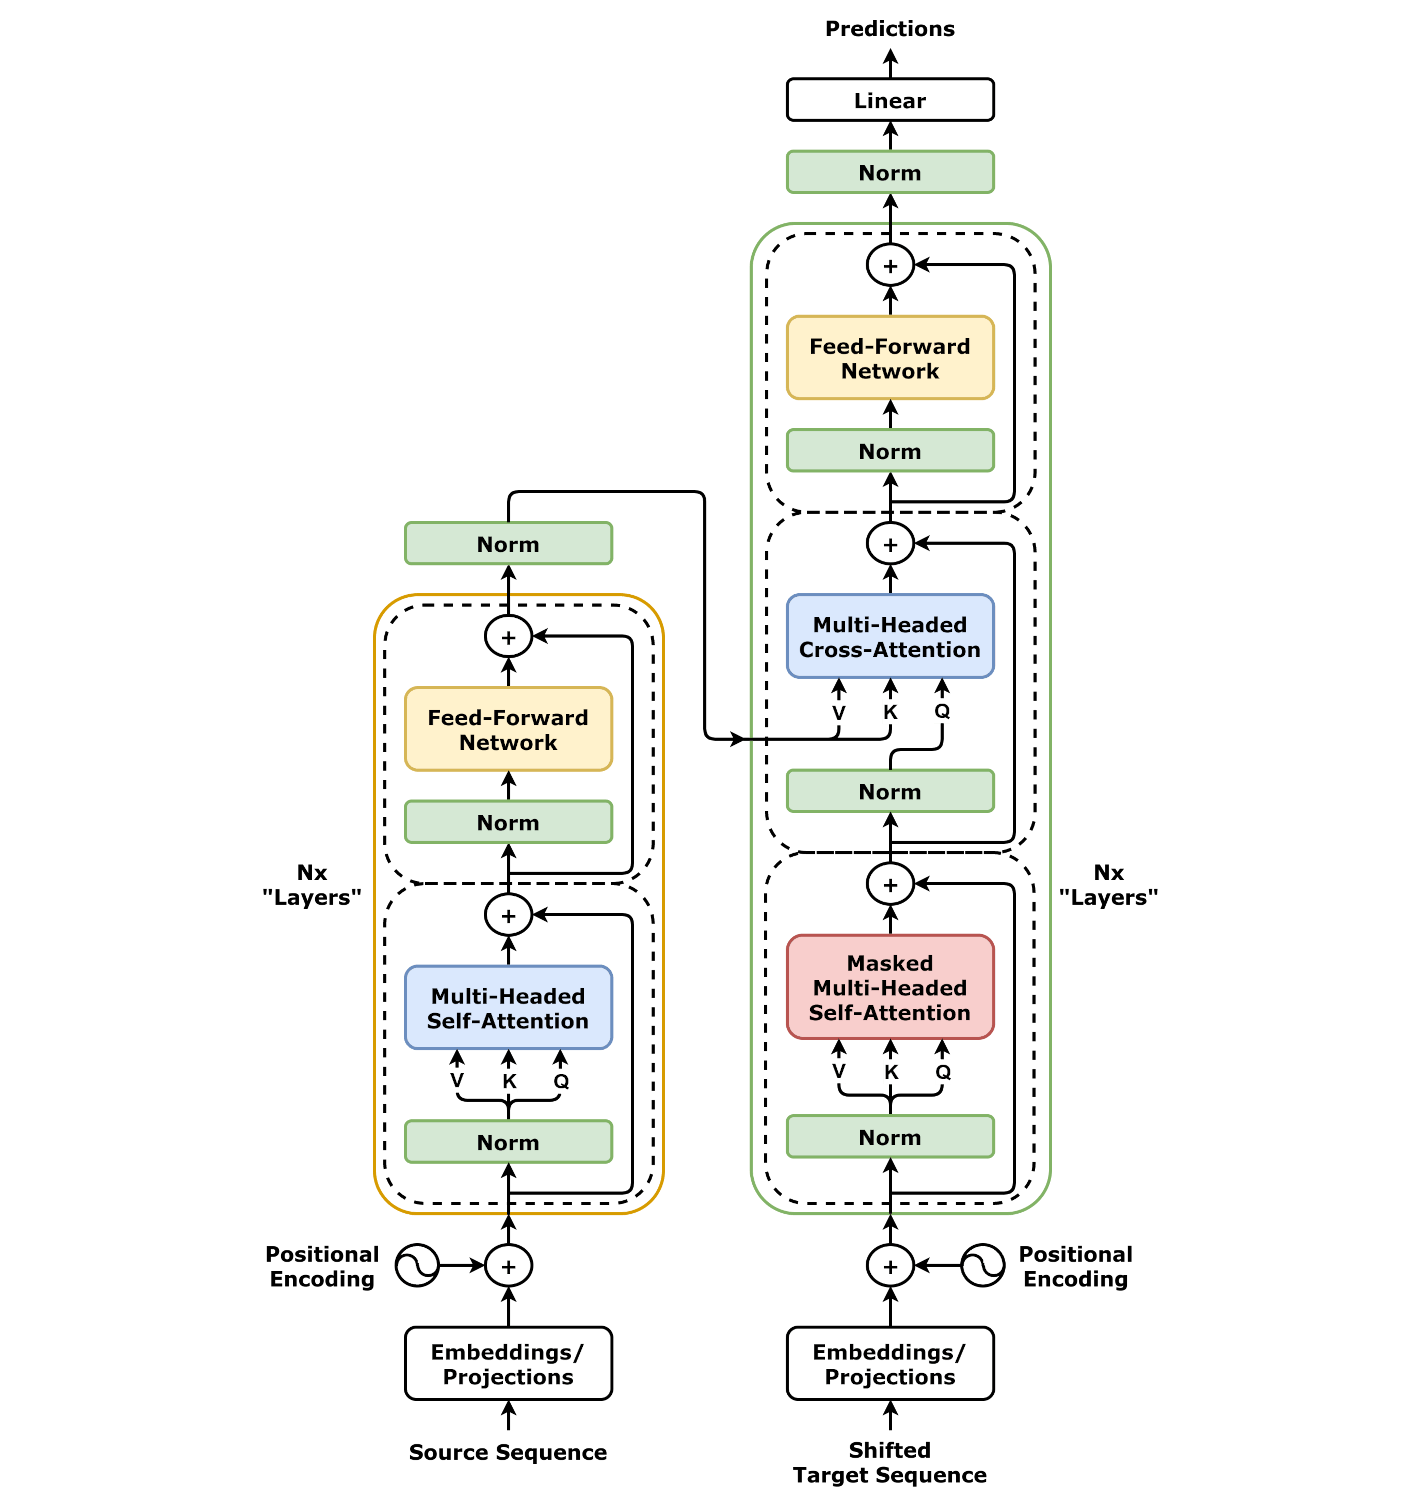
\includegraphics[width=0.8\linewidth]{images/Transformer,_full_architecture.png}
    \caption{Transformer Architecture}
    \label{fig:picture}
\end{figure}

Self-attention computes contextualized token representations by comparing Query, Key, and Value projections:

\[
Q=XW_Q,\quad K=XW_K,\quad V=XW_V
\]
\[
\mathrm{Attention}(Q,K,V)=\mathrm{softmax}\left(\frac{QK^T}{\sqrt{d_k}}\right)V
\]

Each token becomes a weighted combination of value vectors from all tokens.
\begin{itemize}
    \item Before attention, token embeddings are independent.
    \item After attention, each token mixes information from other tokens based on relevance weights.
    \item Intuition: compare ``what I am looking for'' (query) with ``what each token offers'' (key), then aggregate information (value).
\end{itemize}

Cross-attention is used in encoder-decoder models:
\begin{itemize}
    \item Queries come from decoder states.
    \item Keys and values come from encoder outputs.
    \item At each decoding step, the decoder chooses which source tokens matter most.
\end{itemize}



Transformers are attention-based sequence models with strong parallelism.
\begin{itemize}
    \item Input = token embeddings + positional embeddings.
    \item Encoder block: multi-head self-attention, feed-forward network, residual connections, layer norm.
    \item Decoder block: masked self-attention, cross-attention, feed-forward network, residual connections, layer norm.
    \item Output head: linear projection to vocabulary + softmax.
\end{itemize}
Residual structure:
\[
\mathrm{Output}=\mathrm{LayerNorm}(x+\mathrm{SubLayer}(x))
\]
Decoder masking enforces autoregressive next-token prediction.

Transformers are attention-based sequence models with strong parallelism.
\begin{itemize}
    \item Input = token embeddings + positional embeddings.
    \item Encoder block: multi-head self-attention, feed-forward network, residual connections, layer norm.
    \item Decoder block: masked self-attention, cross-attention, feed-forward network, residual connections, layer norm.
    \item Output head: linear projection to vocabulary + softmax.
\end{itemize}
Residual structure:
\[
\mathrm{Output}=\mathrm{LayerNorm}(x+\mathrm{SubLayer}(x))
\]
Decoder masking enforces autoregressive next-token prediction.



\subsection{GPT: Architecture and Training}
GPT is a decoder-only transformer:
\begin{itemize}
    \item Masked self-attention (causal mask) so token $t$ attends only to $\leq t$.
    \item Trained with next-token prediction objective (cross-entropy).
    \item Inference is autoregressive: predict token, append, repeat.
\end{itemize}
Pipeline: tokenization $\rightarrow$ token + positional embeddings $\rightarrow$ stacked decoder blocks $\rightarrow$ linear head + softmax.

\subsection{BERT}
BERT is an encoder-only bidirectional transformer with input:
\[
\text{Token Embedding} + \text{Position Embedding} + \text{Segment Embedding}
\]
BERT input representation details:
\begin{itemize}
    \item WordPiece token embeddings (about 30k vocabulary in the original setup).
    \item Segment embeddings distinguish sentence A vs sentence B.
    \item Position embeddings encode token order.
    \item Special tokens: \texttt{[CLS]} at start and \texttt{[SEP]} between/after sentences.
\end{itemize}
Pretraining objectives:
\begin{itemize}
    \item \textbf{MLM}: predict masked tokens using both left and right context.
    \item \textbf{NSP}: classify whether sentence B follows sentence A.
\end{itemize}
BERT pretraining specifics from your notes:
\begin{itemize}
    \item About 15\% of tokens are selected for MLM.
    \item Of selected tokens: 80\% replaced with \texttt{[MASK]}, 10\% random token, 10\% unchanged.
    \item NSP sampling is typically 50\% true next sentence, 50\% random sentence.
\end{itemize}
BERT workflow has two stages:
\begin{itemize}
    \item \textbf{Pretraining}: self-supervised learning on large unlabeled text.
    \item \textbf{Fine-tuning}: task-specific supervised training with a small task head.
\end{itemize}
BERT model sizes in your notebook:
\begin{itemize}
    \item BERT-base: 12 layers, hidden size 768, 12 heads, around 110M parameters.
    \item BERT-large: 24 layers, hidden size 1024, 16 heads, around 340M parameters.
\end{itemize}
BERT is strong for understanding tasks: classification, NER, QA, and sentence-pair tasks.
\begin{itemize}
    \item Usage tip: with absolute positional embeddings, right-padding is usually preferred.
    \item DistilBERT is a smaller variant with significant speedup and strong retained accuracy.
    \item BERT is excellent for NLU, but decoder models are better suited for free-form generation.
\end{itemize}


\subsection{BART}
BART (Bidirectional and Auto-Regressive Transformers) is a sequence-to-sequence model that combines a bidirectional encoder, similar to BERT, with an autoregressive decoder, similar to GPT. It is designed as a denoising autoencoder for pretraining sequence generation tasks, learning to reconstruct original text from corrupted input.

The architecture is based on the standard Transformer framework. The encoder consists of multiple stacked layers of self-attention and feedforward networks, where each token attends to all other tokens in the input sequence bidirectionally. Formally, given an input sequence \(x = (x_1, x_2, \dots, x_n)\), the encoder produces contextual representations:
\[
h = \text{Encoder}(x).
\]

The decoder is also composed of stacked Transformer layers, but operates autoregressively. Each decoder layer includes masked self-attention, encoder-decoder cross-attention, and feedforward components. At time step \(t\), the decoder generates a token conditioned on previously generated tokens and the encoder output:
\[
p(y_t \mid y_{<t}, x) = \text{Decoder}(y_{<t}, h).
\]

BART is pretrained using a denoising objective. The original input sequence \(x\) is corrupted using a stochastic transformation \(C(x)\), and the model is trained to reconstruct the original sequence:
\[
\mathcal{L} = - \sum_{t} \log p(x_t \mid x_{<t}, C(x)).
\]

Common corruption strategies include token masking, token deletion, text infilling (replacing spans with a mask token), sentence permutation, and document rotation. These transformations force the model to learn both local and global dependencies in the data.

The encoder processes the corrupted input \(C(x)\), producing latent representations:
\[
h = \text{Encoder}(C(x)).
\]
The decoder then generates the original sequence token by token using teacher forcing during training.

The self-attention mechanism in both encoder and decoder is defined as:
\[
\text{Attention}(Q,K,V) = \text{softmax}\left(\frac{QK^T}{\sqrt{d_k}}\right)V,
\]
where \(Q, K, V\) are query, key, and value matrices derived from input embeddings.

The key design of BART lies in combining bidirectional context encoding with left-to-right generation, enabling strong performance across both understanding and generation tasks. After pretraining, the model can be fine-tuned for downstream tasks such as text summarization, machine translation, question answering, and dialogue generation by adapting the decoder output to task-specific formats.


\subsection{T5}
T5 (Text-to-Text Transfer Transformer) is a unified sequence-to-sequence Transformer architecture that reformulates all natural language processing tasks into a text-to-text format. Both inputs and outputs are treated as text strings, enabling a single model to handle diverse tasks such as translation, summarization, classification, and question answering within the same framework.

The architecture follows an encoder-decoder Transformer design. Given an input sequence \(x = (x_1, x_2, \dots, x_n)\), the encoder produces contextual representations:
\[
h = \text{Encoder}(x).
\]
The decoder generates the output sequence \(y = (y_1, y_2, \dots, y_m)\) autoregressively:
\[
p(y_t \mid y_{<t}, x) = \text{Decoder}(y_{<t}, h).
\]

Each layer in both encoder and decoder consists of multi-head attention and position-wise feedforward networks. The attention mechanism is defined as:
\[
\text{Attention}(Q,K,V) = \text{softmax}\left(\frac{QK^T}{\sqrt{d_k}}\right)V.
\]

A distinguishing feature of T5 is its use of a text-to-text paradigm. Every task is converted into a textual input-output pair using task-specific prefixes. For example:
\[
\text{"translate English to German: That is good"} \rightarrow \text{"Das ist gut"}.
\]

T5 is pretrained using a span-corruption objective. Given an input sequence, contiguous spans of tokens are replaced with unique sentinel tokens, and the model is trained to predict the missing spans in order. Let \(C(x)\) denote the corrupted sequence; the objective is:
\[
\mathcal{L} = - \sum_{t} \log p(x_t \mid x_{<t}, C(x)).
\]

Unlike standard masking strategies, the targets consist only of the removed spans, each preceded by its corresponding sentinel token. This allows the model to learn structured reconstruction and long-range dependencies.

T5 uses relative position embeddings instead of absolute positional encodings, improving generalization to longer sequences. The model is trained on a large-scale dataset (C4: Colossal Clean Crawled Corpus), emphasizing transfer learning across tasks.

During fine-tuning, no architectural changes are required. Tasks are specified purely through input text formatting, and the model generates outputs accordingly. This unified formulation simplifies the pipeline and enables strong performance across a wide range of NLP benchmarks.



\subsection{Generative Adversarial Networks}

Generative Adversarial Networks (GANs) are a class of generative models that learn to approximate a target data distribution by framing the learning problem as a two-player minimax game. The framework consists of two neural networks: a generator \(G\) and a discriminator \(D\), both parameterized by differentiable functions.

The generator \(G(z)\) maps a latent variable \(z \sim p_z(z)\), typically drawn from a simple prior such as a standard normal distribution, into the data space. Its objective is to produce samples that resemble the true data distribution \(p_{\text{data}}(x)\). The discriminator \(D(x)\) outputs a scalar in \([0,1]\), representing the probability that input \(x\) is drawn from the real data rather than generated.

The interaction between these two networks is formalized as a minimax optimization problem:
\[
\min_G \max_D \; V(D,G)
\]
where the value function is given by
\[
V(D,G) = \mathbb{E}_{x \sim p_{\text{data}}(x)}[\log D(x)] + \mathbb{E}_{z \sim p_z(z)}[\log(1 - D(G(z)))].
\]

The discriminator seeks to maximize this objective by correctly classifying real samples as real and generated samples as fake. Conversely, the generator seeks to minimize the same objective by producing samples that maximize the discriminator's error.


\section{BLEU Score (Bilingual Evaluation Understudy)}

BLEU is a corpus-level metric for evaluating generated text by comparing it with one or more reference texts. It is primarily based on \textbf{modified n-gram precision} with a \textbf{brevity penalty} to discourage overly short outputs.


\[
\text{BLEU} = BP \cdot \exp \left( \sum_{n=1}^{N} w_n \log p_n \right)
\]

\begin{itemize}
    \item $p_n$: modified precision for n-grams
    \item $w_n$: weights (typically uniform, e.g., $w_n = \frac{1}{N}$)
    \item $BP$: brevity penalty
\end{itemize}

\subsection{Modified n-gram Precision}

\[
p_n =
\frac{\sum\limits_{\text{n-grams}} \min(\text{count}_{\text{cand}}, \text{count}_{\text{ref}})}
{\sum\limits_{\text{n-grams}} \text{count}_{\text{cand}}}
\]

\textbf{Intuition:}
\begin{itemize}
    \item Measures: ``How many generated n-grams are correct?''
    \item Denominator = total candidate n-grams
    \item Numerator = matching n-grams (with clipping)
\end{itemize}

\subsection{Clipping}

Each n-gram match is \textbf{capped} by its maximum frequency in the reference:
\[
\text{count}_{\text{clip}} = \min(\text{count}_{\text{cand}}, \text{count}_{\text{ref}})
\]

This prevents artificially inflating precision by repetition.


If a sentence has $N$ tokens, the number of n-grams is:
\[
N - n + 1
\]

\begin{itemize}
    \item Unigram ($n=1$): $N$
    \item Bigram ($n=2$): $N-1$
    \item Higher $n$: stricter matching
\end{itemize}

\subsection{Brevity Penalty (BP)}

\[
BP =
\begin{cases}
1 & \text{if } c > r \\
e^{(1 - r/c)} & \text{if } c \le r
\end{cases}
\]

\begin{itemize}
    \item $c$: candidate length
    \item $r$: reference length
\end{itemize}

\textbf{Behavior:}
\begin{itemize}
    \item If $c < r$: $BP < 1$ (penalty applied)
    \item As $c \ll r$: $BP \to 0$ (strong penalty)
    \item If $c > r$: $BP = 1$ (no penalty)
    \item Precision-based (no recall)
    \item Uses geometric mean across n-grams
    \item Penalizes short outputs via $BP$
    \item Sensitive to exact wording (not semantics)
\end{itemize}

\section{BERTScore}

BERTScore is a metric for evaluating generated text using \textbf{contextual embeddings} from transformer models (e.g., BERT). Instead of exact n-gram overlap, it measures \textbf{semantic similarity} between candidate and reference tokens.

Each token in the candidate and reference is mapped to a contextual embedding. Similarity between tokens is computed using cosine similarity, allowing matching of \textbf{paraphrases and semantically similar words}.


Let:
\begin{itemize}
    \item $\mathbf{x}_i$: embedding of $i$-th candidate token
    \item $\mathbf{y}_j$: embedding of $j$-th reference token
\end{itemize}

\[
\text{sim}(\mathbf{x}_i, \mathbf{y}_j) = \frac{\mathbf{x}_i \cdot \mathbf{y}_j}{\|\mathbf{x}_i\| \|\mathbf{y}_j\|}
\]

\subsection{BERT Precision}

\[
P_{\text{BERT}} =
\frac{1}{|x|} \sum_{i=1}^{|x|} \max_{j} \ \text{sim}(\mathbf{x}_i, \mathbf{y}_j)
\]

\textbf{Intuition:}
\begin{itemize}
    \item For each candidate token, find the \textbf{most similar} token in the reference
    \item Average these similarities
\end{itemize}

\textbf{Interpretation:}
\begin{itemize}
    \item ``How much of the generated text is semantically correct?''
\end{itemize}

\subsection{BERT Recall}

\[
R_{\text{BERT}} =
\frac{1}{|y|} \sum_{j=1}^{|y|} \max_{i} \ \text{sim}(\mathbf{x}_i, \mathbf{y}_j)
\]

\textbf{Intuition:}
\begin{itemize}
    \item For each reference token, find the \textbf{best matching} token in the candidate
    \item Average these similarities
\end{itemize}

\textbf{Interpretation:}
\begin{itemize}
    \item ``How much of the reference meaning is captured by the generated text?''
\end{itemize}


\begin{itemize}
    \item Captures \textbf{semantic similarity}, not exact matches
    \item Handles \textbf{paraphrases and synonyms}
    \item Token-level alignment via \textbf{maximum similarity matching}
    \item Uses contextual embeddings (context-dependent meaning)
    \item BLEU: surface-level n-gram precision
    \item BERTScore: embedding-based semantic similarity
    \item BLEU fails on paraphrases; BERTScore handles them better
\end{itemize}

\section{ROUGE Score (Recall-Oriented Understudy for Gisting Evaluation)}

ROUGE is a set of metrics used to evaluate generated text (e.g., summaries) by comparing it with reference text(s). Unlike BLEU, ROUGE is primarily \textbf{recall-oriented}, focusing on how much of the reference content is captured by the candidate.


ROUGE measures \textbf{overlap between candidate and reference}, typically using:
\begin{itemize}
    \item n-grams (ROUGE-N)
    \item longest common subsequence (ROUGE-L)
\end{itemize}

\subsection{ROUGE-N (n-gram Recall)}

\[
\text{ROUGE-N} =
\frac{\sum\limits_{\text{n-grams}} \min(\text{count}_{\text{cand}}, \text{count}_{\text{ref}})}
{\sum\limits_{\text{n-grams}} \text{count}_{\text{ref}}}
\]

\textbf{Intuition:}
\begin{itemize}
    \item Measures: ``How much of the reference n-grams are recovered by the candidate?''
    \item Numerator = overlapping n-grams (with clipping)
    \item Denominator = total n-grams in the reference
\end{itemize}

\subsection{ROUGE Precision (optional)}

\[
P_{\text{ROUGE-N}} =
\frac{\sum\limits_{\text{n-grams}} \min(\text{count}_{\text{cand}}, \text{count}_{\text{ref}})}
{\sum\limits_{\text{n-grams}} \text{count}_{\text{cand}}}
\]

\textbf{Interpretation:}
\begin{itemize}
    \item ``How much of the generated content is relevant?''
\end{itemize}


If a sequence has $N$ tokens, the number of n-grams is:
\[
N - n + 1
\]

\subsection{ROUGE-L (Longest Common Subsequence)}

ROUGE-L is based on the \textbf{Longest Common Subsequence (LCS)}, which captures sentence-level structure without requiring consecutive matches.

\[
R_{\text{LCS}} = \frac{\text{LCS}(x,y)}{|y|}
\quad\quad
P_{\text{LCS}} = \frac{\text{LCS}(x,y)}{|x|}
\]

\[
F1_{\text{LCS}} =
\frac{2 \cdot P_{\text{LCS}} \cdot R_{\text{LCS}}}
{P_{\text{LCS}} + R_{\text{LCS}}}
\]

\textbf{Intuition:}
\begin{itemize}
    \item Captures in-order matching (not necessarily contiguous)
    \item Rewards fluency and structure better than pure n-grams
\end{itemize}










\end{document}